\documentclass[a4paper,10pt]{article}
\usepackage[utf8]{inputenc}
\usepackage{graphicx}
\usepackage{listings}
\usepackage{physics}
\usepackage[margin=1in]{geometry}
\usepackage{subcaption}


\lstset{basicstyle=\footnotesize, breaklines = false}

\date{\today}
\title{FYS-MENA4111 - lab report 1}
\author{Mikael B. Kiste}

\begin{document}
  \maketitle
  \tableofcontents

  \newpage
  \section{Introduction}
    In this laboratory assignment we got an introduction in how to navigate in the terminal to access the Abel supercomputer and run our simulations.
    There are quite a number of useful commands, some new to me and some I was used to.
    Once inside Abel we had access to some files with parameters and initial conditions of bulk Silicon (diamond cubic crystal structure) to get us started on looking at DFT calculations. The 'more' command easily shows the contents of a text file, while files containing information about the crystal structure can be opened in vesta. There are five important input files that are needed before simulations are started: POSCAR, INCAR, KPOINTS, POTCAR and the job script.
    \begin{itemize}
      \item POSCAR: This is the main file as it defines the crystal structure of your system that you are looking at. It contains the \textbf{positions} of the atoms in the unit cell. It is possible to open this file in VESTA to get an impression of the spatial coordination of the atoms. 
      \item INCAR: Arguments and parameters that are defining for the simulation are contained in this \textbf{in} file. One important parameter is the criterion for self-consistence (in eV). Between iterations the program will only proceed if the calculated total energy is less than this value.
      \item KPOINTS: The \textbf{k-points} in reciprocal space are defined in this file as they are needed for the numerical integrations in the program.
      \item POTCAR: The POTCAR file is also of importance as it concerns the \textbf{potential} or, more specifically, the exchange-correlation functional.
      \item jobfile: This is the actual file that is run (through the \texttt{sbatch} command) from the terminal to start the calculation \textbf{job}.
    \end{itemize}
	Since this is the first laboratory exercise we did not manipulate these input files. Later in the course this aspect will be covered in more depth.
  	\begin{figure}[h]
		\centering
		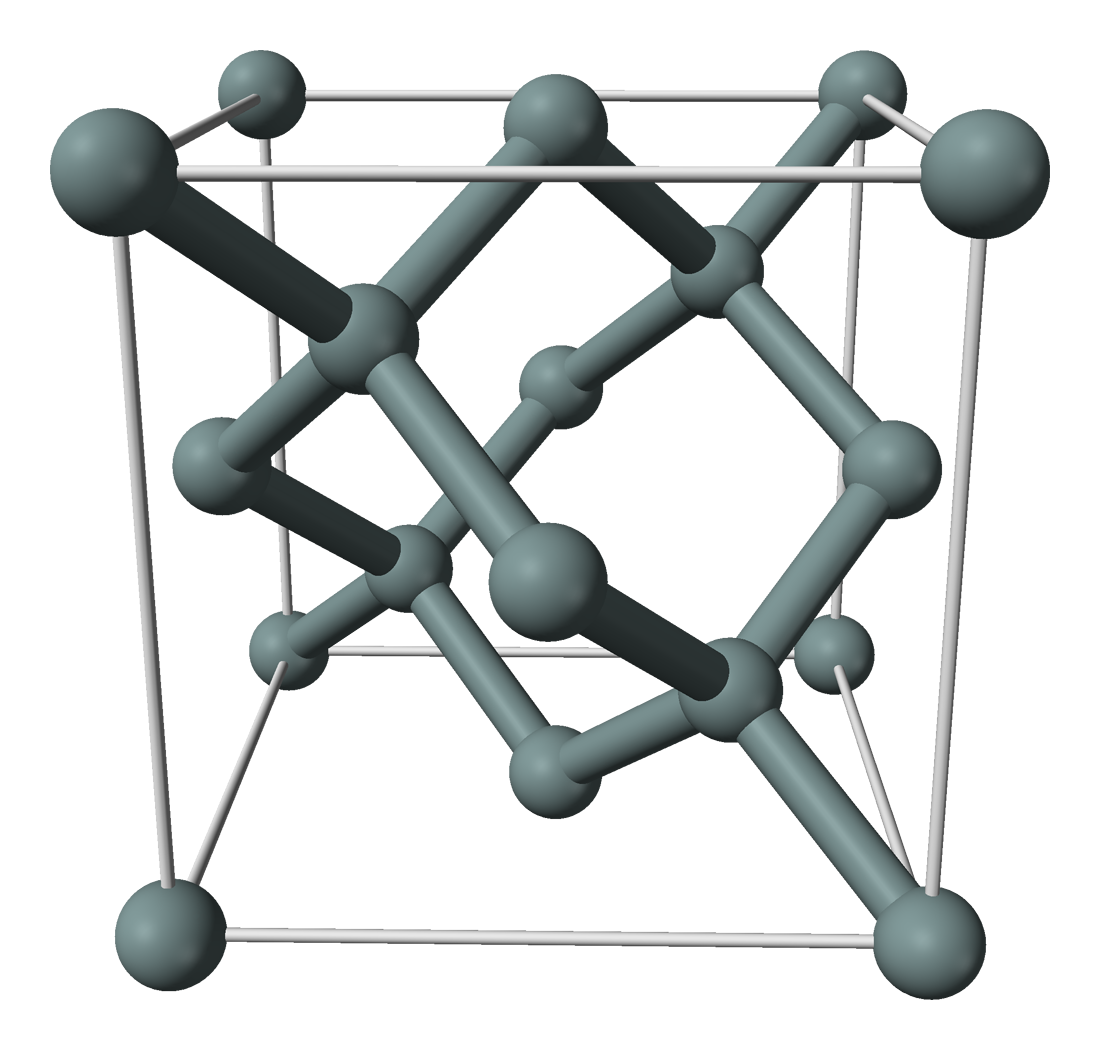
\includegraphics[width=0.7\linewidth]{SiCell}
		\caption{Silicon crystallizes in a diamond cubic crystal structure (from the wikipedia page on Silicon). It consists of the fcc crystal structure but with the addition of four tetrahedrally coordinated atoms within the cell}
		\label{fig:sicell}
	\end{figure}
	
	\newpage
    \section{Information from the output files}
    After the job has finished and the calculations are completed there will be some output files generated:
    \begin{itemize}
    	\item OSZICAR: It's a good idea to check the contents of OSZICAR after every simulation. The data indicates whether or not the job has converged properly. For every iteration that was needed it prints both $\dd E$ and $\dd \epsilon$, both of which should converge and be less than the limit defined in the INCAR file in the last iteration. Total electronic energy $E0$ is displayed at the bottom after self-consistence has been achieved .
    	\item slurm-JOBID.out: A simple file containing any error messages that might have been produced
    	\item OUTCAR: The main output file containing a lot of information about the job. Using the \texttt{vaspout} command on the file will print some properties that are always of interest. It includes \texttt{TOTEN}, the energy difference between infinitely separated atoms and the crystal structure specified in POSCAR (excluding temperature effects, therefore representing the total \textit{electronic} energy).
    	\item vasprun.xml: machine-readable format of OUTCAR
    	\item CHGCAR: This file contains the \textbf{charge} density of the relaxed system. This file can also be opened in VESTA, giving an impression of bonds and electron density in general.
    \end{itemize}
	\begin{figure}[h]
	\begin{center}
		\begin{subfigure}{0.4\textwidth}
			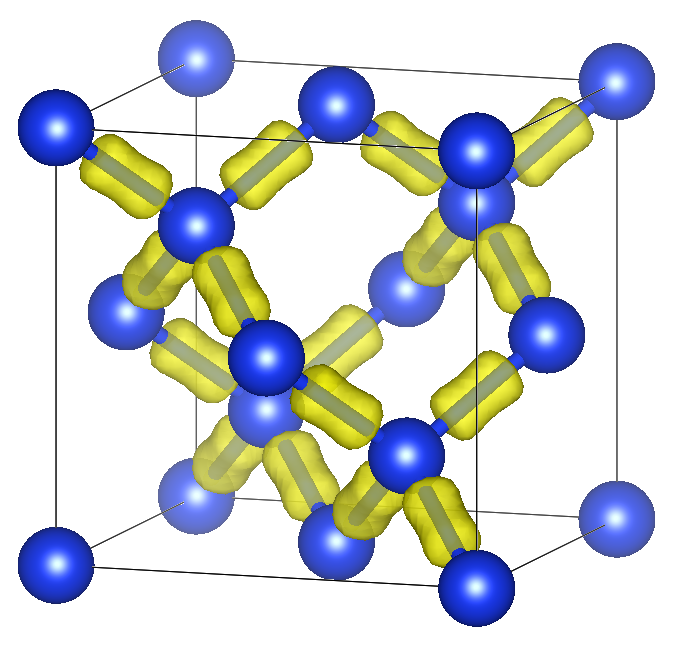
\includegraphics[width=1.0\linewidth]{si_bulk/chg1.png} 
			\caption{Ball and stick model including regions\\of high electron density in yellow}
			\label{fig:subim1}
		\end{subfigure}
		\begin{subfigure}{0.4\textwidth}
			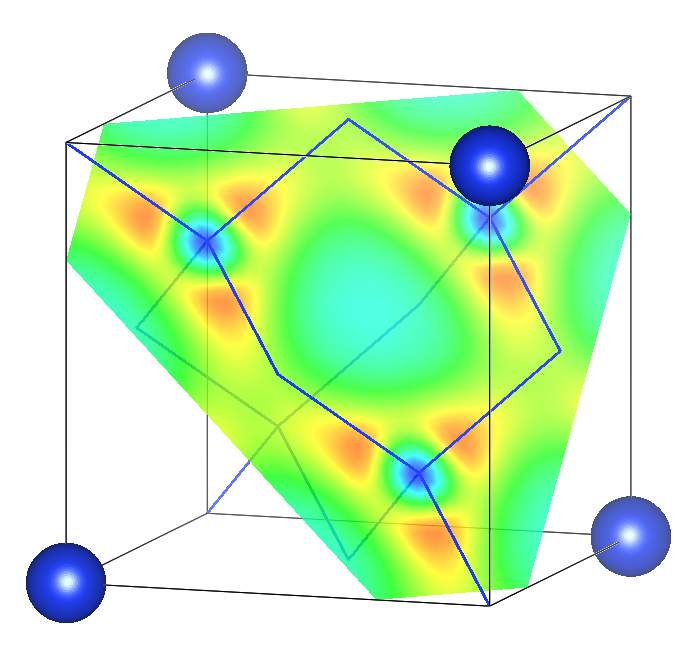
\includegraphics[width=1.0\linewidth]{si_bulk/chg2.png}
			\caption{Wireframe model with charge density\\displayed in the [1,1,1] lattice plane}
			\label{fig:subim2}
		\end{subfigure}
		
		\caption{VESTA can generate many different illustrations of the crystal structure and electron density based on the same CHGCAR file. In figure \ref{fig:subim2} you can see the charge density in the plane of three of the four intra-cell atoms. This plane is perpendicular to the excluded intra-cell atom and therefore only indicates three of the four bonds}
		\label{fig:image2}
	\end{center}
	\end{figure}
	\newpage
    \subsection{Slurm file error messages}
      For every job run there is also a slurm file created that contains any error messages that may have been encountered. The slurm file for this exercise is included in the appendix. With the exception of two minor alerts the program seemed to run just fine. A warning directed at users running VASP/VAMP was instantiated. Apparently it is recommended to use the reciprocal-space projection scheme for small supercells as this is both more efficient and accurate. There is also a warning of possible aliasing (wrap around) errors thrown.
      
    \subsection{The results in OUTCAR}
    Calling on OUTCAR with the \texttt{vaspout} command returns the following:\\
	\begin{center}
    \begin{tabular}{ccccc}
    	\texttt{MxForce} & \texttt{Drift} & \texttt{Press} & \texttt{TOTEN} & \texttt{Filename} \\
    	\texttt{0.000} & \texttt{0.000} & \texttt{18.02} & \texttt{-43.297736} & \texttt{OUTCAR} \\
    \end{tabular}
	\end{center}
	Using the \texttt{grep} command makes searching through the large OUTCAR file easier. The supercell consists of four primitive cells. There were 10 irreducible k-points. Shortest nearest neighbor distance was 2,35Å. The number of bands was 21 and the number of plane waves was 13824. Total CPU time used was 3.384 seconds and maximum memory used was 30 272kb.

	\section{Conclusion}
	In conclusion using Abel to do DFT simulations seems pretty straight forward, as long as one knows the basic commands. Calculations are pretty fast on this supercomputer and both the input and output files are neatly organized. The most important (and trickiest) aspect is probably correctly interpreting the data (including what assumptions are made in the model) and tweaking the input arguments to get the best possible description of your material.

	\newpage
	\appendix
	\section{appendix}
	\subsection{Slurm file}
	    \lstinputlisting{si_bulk/slurm-23047367.out}
	\newpage
	\subsection{OSZICAR file}
		\lstinputlisting{si_bulk/OSZICAR.txt}
\end{document}
